%%%%%%%%%%%%%%%%%%%%%%%%%%%%%%%%%%%%%%%%%%%%%%%%%%%%%%%%%%%%%%%%%%%%%%%%%%%%%%%%%%%%%%%%%%%%%%%%%%%%%%%%%%%%%%%%%%%%%%%%%%%%%%%%%%%%%%%%%%%%%%%%%%%%%%%%%%%%%%%%%%%
% Written By Michael Brodskiy
% Class: Fundamentals of Electronics
% Professor: M. Onabajo
%%%%%%%%%%%%%%%%%%%%%%%%%%%%%%%%%%%%%%%%%%%%%%%%%%%%%%%%%%%%%%%%%%%%%%%%%%%%%%%%%%%%%%%%%%%%%%%%%%%%%%%%%%%%%%%%%%%%%%%%%%%%%%%%%%%%%%%%%%%%%%%%%%%%%%%%%%%%%%%%%%%

\include{Includes.tex}

\title{Lecture 1}
\date{September 4 — \today}
\author{Michael Brodskiy\\ \small Professor: M. Onabajo}

\begin{document}

\maketitle

\begin{itemize}

  \item Broad circuit categories:

    \begin{itemize}

      \item Information processing $\to$ cell phone, GPS, cable TV

      \item Power delivery $\to$ AC-to-DC power adapter, power amplifiers, EVs

    \end{itemize}

  \item Applications

    \begin{itemize}

      \item Communication systems

      \item Medical electronics

      \item Computers (digital signal processing)

      \item Instrumentation

      \item Control systems

      \item Power systems

      \item Toys

    \end{itemize}

  \item Electronic circuits that are manufactured as integrated circuits (ICs)

    \begin{itemize}

      \item ``Chips'' — created with semiconductor device fabrication processes

    \end{itemize}

  \item Semiconductor Industry

    \begin{itemize}

      \item 1947

        \begin{itemize}

          \item First transistor was invented at Bell Laboratories by William Shockley, John Bardeem, and Walter Brattain

          \item ``The basis of modern electronics''

        \end{itemize}

      \item 1958 — 1961

        \begin{itemize}

          \item Introduction of the integrated circuit by Jack Kilby (Texas Instruments) and Robert Noyce (Fairchild Semiconductor)

          \item Enabled miniaturization and mass production of chips

        \end{itemize}

      \item Today

        \begin{itemize}

          \item Smallest dimensions of features in the silicon around 5 [nm]

          \item Up to $>$2.5 billion transistors per chip

          \item $>$\$300 billion global revenue

        \end{itemize}

    \end{itemize}

  \item Course Overview

    \begin{itemize}

      \item Amplifier concepts

      \item Study of electronic devices

        \begin{itemize}

          \item Operational amplifiers (Op-Amps)

          \item Diodes

          \item Bipolar junction transistors (BJTs)

          \item Metal-oxide-semiconductor field effect transistors (MOSFETs)

        \end{itemize}

      \item Design and analysis of electronic circuits

        \begin{itemize}

          \item Analog amplifiers, rectifier circuits

          \item Digital logic

        \end{itemize}

    \end{itemize}

  \item Main Course Goals

    \begin{itemize}

      \item Understand the operation of fundamental electronic devices (op-amps, diodes, BJTs, MOSFETs)

      \item Analyze and design operational amplifier circuits and rectifier circuits

      \item Analyze and design amplifiers with BJTs and MOSFETs

      \item Be able to identify CMOS logic circuits (NOT, NAND, NOR), and analyze voltage transfer curves and propagation delays

      \item Simulate electronic circuits using PSPICE

    \end{itemize}

  \item Review — Some Circuit Analysis Highlights

    \begin{itemize}

      \item Element combination rules (parallel, serial)

      \item Ohm's Law: $I=V/R$

      \item KVL for a circuit loop $\to \sum_jv_j=0$

      \item KCL at a node $\to\sum_ji_j=0$

      \item Superposition principle

        \begin{itemize}

          \item If input A produces response X and input B produces response Y, then input (A+B) produces response (X+Y)

          \item Holds only for linear circuits

          \item Very useful for circuits with multiple voltage and current sources

        \end{itemize}

      \item Th\'evenin and Norton form of signal sources

        \begin{itemize}

          \item Valid only in linear circuits

        \end{itemize}

    \end{itemize}

  \item Element Combination Rules

    \begin{itemize}

      \item Resistors in series can be summed ($R_1+R_2+\cdots+R_n=R_t$)

      \item Resistors in parallel can be summed via conductances $\left( G_x=\frac{1}{R_x}\right)$ can be combined to get $\to G_1+G_2+\cdots+G_n=G_t$

      \item Voltages in series can be summed ($V_1+V_2+\cdots+V_n=V_t$)

      \item Voltages in parallel will not occur, as it is illogical to place them in such a manner (and is the same reason current sources in series do not occur)

      \item Current sources in parallel may be summed ($i_1+i_2+\cdots+i_n=i_t$)

    \end{itemize}

  \item Analysis of Large Circuits

    \begin{itemize}

      \item Write all expressions for the circuit

        \begin{itemize}

          \item At elements (Ohm's Law)

          \item At nodes (KCL)

          \item For loops (KVL)

        \end{itemize}

      \item Eliminate redundant equations (keep only independent equations)

      \item Solve the system of equations for the unknown variables

    \end{itemize}

  \item Th\'evenin and Norton Equivalent Representations

    \begin{itemize}

      \item Th\'evenin to Norton transformation

        \begin{itemize}

          \item Set $I_s=V_s/R_s$ (short-circuit current), and $R_P=R_s$

        \end{itemize}

      \item Norton to Th\'evenin transformation

        \begin{itemize}

          \item Set $V_s=I_sR_s$ (open-circuit voltage), and $R_s=R_P$

          \end{itemize}

      \item In more complex cases, $R_s$ and $R_P$ are the equivalent resistances seen at terminals

    \end{itemize}

  \item A circuit can be broken into ``source'' components by assuming an open circuit for current sources, and short circuit for voltage sources

  \item This gives us components which we can then sum up via the superposition principle:

    \begin{figure}[H]
      \centering
      \include{Figures/Lec1Circuit}
      \caption{Initial Circuit}
      \label{fig:1}
    \end{figure}

    \begin{figure}[H]
      \centering
      \tikzset{every picture/.style={line width=0.75pt}} %set default line width to 0.75pt        

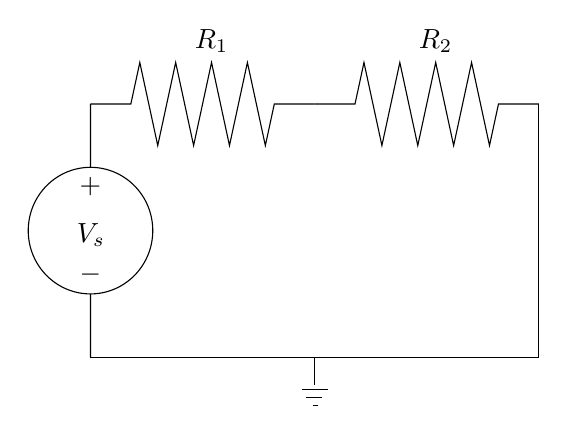
\begin{tikzpicture}[x=0.75pt,y=0.75pt,yscale=-1,xscale=1]
%uncomment if require: \path (0,300); %set diagram left start at 0, and has height of 300

%Shape: Output [id:dp694152168500714] 
\draw   (139,119.5) .. controls (155.57,119.5) and (169,133.16) .. (169,150) .. controls (169,166.84) and (155.57,180.5) .. (139,180.5) .. controls (122.43,180.5) and (109,166.84) .. (109,150) .. controls (109,133.16) and (122.43,119.5) .. (139,119.5) -- cycle (139,89) -- (139,119.5) (139,211) -- (139,180.5) ;
%Shape: Resistor [id:dp014514785173657008] 
\draw   (139,89) -- (158.44,89) -- (162.76,69) -- (171.4,109) -- (180.04,69) -- (188.68,109) -- (197.32,69) -- (205.96,109) -- (214.6,69) -- (223.24,109) -- (227.56,89) -- (247,89) ;
%Shape: Resistor [id:dp6346068220663863] 
\draw   (247,89) -- (266.44,89) -- (270.76,69) -- (279.4,109) -- (288.04,69) -- (296.68,109) -- (305.32,69) -- (313.96,109) -- (322.6,69) -- (331.24,109) -- (335.56,89) -- (355,89) ;
%Straight Lines [id:da8900340649133313] 
\draw    (139,211) -- (355,211) ;
%Straight Lines [id:da802632819816991] 
\draw    (355,89) -- (355,211) ;
%Straight Lines [id:da37478191641684244] 
\draw    (247,211) -- (247,224.42) ;
%Straight Lines [id:da6053270148706792] 
\draw    (253.42,226.42) -- (241,226.42) ;
%Straight Lines [id:da08135722826593528] 
\draw    (250.42,230.42) -- (243,230.42) ;
%Straight Lines [id:da9692312024110025] 
\draw    (248.42,234.42) -- (246,234.42) ;

% Text Node
\draw (139,122.9) node [anchor=north] [inner sep=0.75pt]    {$+$};
% Text Node
\draw (139,177.1) node [anchor=south] [inner sep=0.75pt]    {$-$};
% Text Node
\draw (139.2,152.19) node    {$V_{s}$};
% Text Node
\draw (197.32,65.6) node [anchor=south] [inner sep=0.75pt]    {$R_{1}$};
% Text Node
\draw (305.32,65.6) node [anchor=south] [inner sep=0.75pt]    {$R_{2}$};


\end{tikzpicture}

      \caption{Voltage Component}
      \label{fig:2}
    \end{figure}

    \begin{figure}[H]
      \centering
      \include{Figures/Lec1CircuitI}
      \caption{Current Component}
      \label{fig:3}
    \end{figure}

  \item Amplification

    \begin{itemize}

      \item Voltage gain: $|A_v|$

        \begin{itemize}

          \item When $|A_v|$ is constant: linear amplifier

          \item When $|A_v|$ is not constant: non-linear amplifier

        \end{itemize}

      \item Non-inverting amplifier: $v_o(t)=A_vv_i(t)$

      \item Inverting amplifier: $v_o(t)=-A_vv_i(t)$

    \end{itemize}

  \item Voltage-Amplifier Model

    \begin{itemize}

        \begin{figure}[H]
          \centering
          \includegraphics[width=.7\textwidth]{Images/VAM.png}
          \caption{Reference Figure for the Voltage-Amplifier Model}
          \label{fig:4}
        \end{figure}

      \item Parameters

        \begin{itemize}

          \item $v_s$ is the input voltage source, which has a series resistance $R_s$

          \item $R_i$ and $R_o$ are the input and output resistances, respectively

          \item $A_{vo}$ is the open-circuit voltage gain

          \item $R_L$ is the load resistance

        \end{itemize}

      \item Remember: This is a simplified representation of an amplifier

      \item Current gain: $A_i=\dfrac{i_o}{i_i}=\dfrac{(v_o/R_L)}{(v_i/R_i)}=A_v(R_i/R_L)$

      \item Loaded voltage gain: $A_v=\dfrac{v_o}{v_i}\neq A_{vo}$

      \item Power gain: $G=\dfrac{P_o}{P_i}=\underbrace{\dfrac{V_oI_o}{V_iI_i}}_{\text{RMS}}=A_vA_i=A_v^2\cdot\dfrac{R_i}{R_L}$

      \item For optimum voltage transfer, $R_L>>R_o$

    \end{itemize}

  \item Loading Effects

    \begin{itemize}

      \item Refer to the same figure (Figure \ref{fig:4}) as for the Voltage-Amplifier Mode

      \item Input signal attentuation: $v_i=v_s\left( \dfrac{R_i}{R_i+R_s} \right)$

      \item Output signal attentuation: $v_o=A_{vo}v_i\left( \dfrac{R_L}{R_L+R_o} \right)$

      \item Loaded voltage gain of the amplifier: $A_v=\dfrac{v_o}{v_i}=A_{vo}\left( \dfrac{R_L}{R_L+R_o} \right)$

      \item Voltage gain from source to load $A_{vs}=\frac{v_o}{v_s}=A_{vo}\left( \dfrac{R_i}{R_i+R_s} \right)\left( \dfrac{R_L}{R_L+R_o} \right)$

    \end{itemize}

  \item Decibel Notation

    \begin{itemize}

      \item Use $20\log(X)$ for voltages and currents

        \begin{itemize}

          \item $A_{v\text{dB}}=20\log(|A_v|)$

          \item $A_{i\text{dB}}=20\log(|A_i|)$

        \end{itemize}

      \item Use $10\log(X)$ for powers

        \begin{itemize}

          \item $G_{\text{dB}}=10\log(|G|)$

        \end{itemize}

      \item Quantities in decibels are added when two or more amplifiers are connected in series (called ``cascaded'')

    \end{itemize}

\end{itemize}

\end{document}

